\section{Fourier Transformation}

We have already seen the problem of aliasing. Now we want to understand how we can avoid aliasing and for this we introduce the \textbf{Fourier Transformation}. \medskip

The idea behind the Fourier transformation is to perform a change of basis, where the new basis elements are of the form $e^{-i2\pi (ux + vy)} = \cos (2 \pi (ux + vy)) - i \sin (2 \pi (ux + vy))$ (u, v are the parameters for the new basis).
$$F(g(x,y))(u,v) = \int \int_{R^2} g(x,y) e^{-i2\pi (ux + vy)} dxdy$$

The basis functions of Fourier transform are eigenfunctions of linear systems (one of the reasons it is so popular). Discrete Fourier transformation (DFT) can be represented as:
$$F = \textbf U f$$

Here $\textbf U$ is the Fourier transform base. The vector $(u,v)$ determines the frequency by its magnitude and the orientation by its direction (only looking at the real part):
\begin{center}
	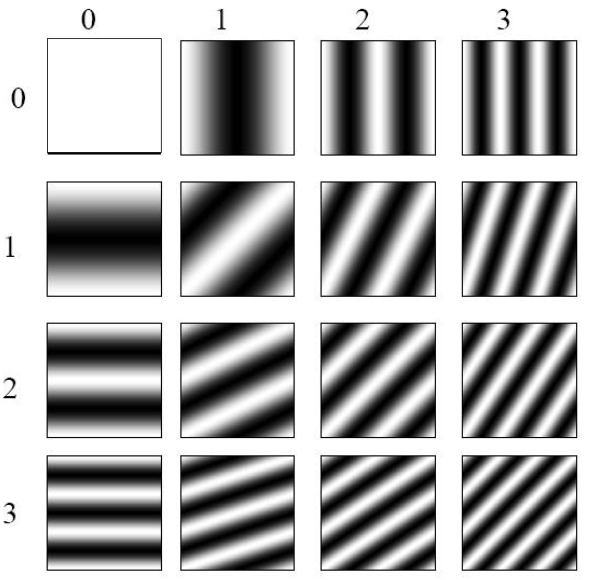
\includegraphics[width=0.6\linewidth]{fourier_transform_pattern.png}
\end{center}


\subsection{Phase and Magnitude}

Since the Fourier transform is complex, it is difficult to plot. Instead we think of the phase (angle) and magnitude (length of the vector) of the transform. Note that natural images have about the same magnitude transform, hence phase seems to matter more. The phase part seems more random than the magnitude. Here you can see an example of the magnitude of an image.
\begin{center}
	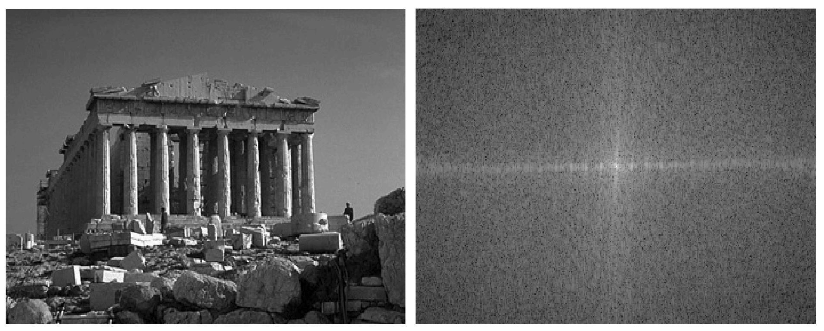
\includegraphics[width=\linewidth]{phase_magnitude.png}
\end{center}


\subsection{Properties of the Fourier Transform}

We already said that the Fourier transform is linear. Further it is important to note that the FT of a Gaussian is a Gaussian. 
\begin{center}
	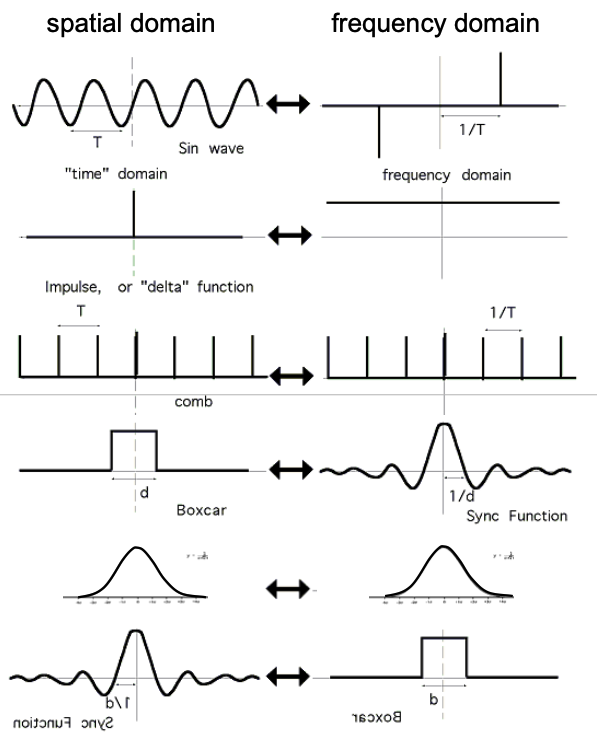
\includegraphics[width=0.7\linewidth]{ft_examples.png}
\end{center}

\textbf{Convolution Theorem} \smallskip

The FT of the convolution of two functions is the product of their FT and the other way around:
$$F \cdot G = \textbf U (f * g), \qquad F * G = \textbf U (f \cdot g)$$


\subsection{Sampling}

Now we have a look at aliasing again. We define our sampling function as follows:
$$\text{Sample}_{2 \text D} (f(x,y)) = f(x,y) \sum_{i = - \infty}^\infty \sum_{j = - \infty}^\infty \delta (x-i, y-j)$$

Where $\delta$ is the Dirac delta function. The FT of a sampled signal now corresponds to:
$$F(\text{Sample}_{2 \text D} (f(x,y)))) = \sum_{i = - \infty}^\infty \sum_{j = - \infty}^\infty F(u-i, v-i)$$

This approach can still lead to aliasing as high frequencies can lead to trouble. To avoid this we first need to suppress high frequencies before sampling. We can do this by convolution with a low-pass filter, this corresponds to multiplying the FT with the same filter. As a low-pass filter we use a Gaussian. \medskip

\textbf{Nyquist Sampling Theorem} \smallskip

To understand why we need to do the low-pass filtering, we can take a look at the Nyquist sampling theorem: \textit{The sampling frequency must be at least twice the highest frequency (of the signal)}.


\subsection{Signal Reconstruction}

In image reconstruction we want to recreate our image from the samples data. To avoid pixelation we look at different reconstruction filters.
\begin{center}
	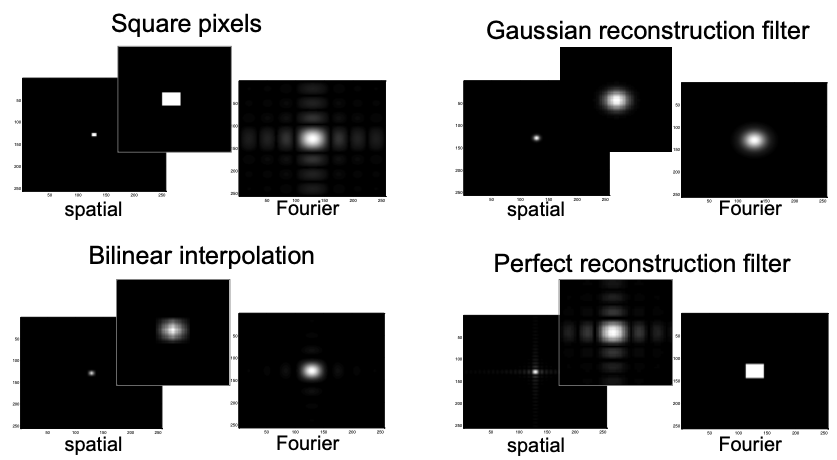
\includegraphics[width=\linewidth]{reconstruction.png}
\end{center}

In the Fourier domain, determining the inverse of a kernel / filter becomes a lot easier, as:
$$F(h)(u,v) \cdot F(h^{-1})(u,v) = 1$$

With this we can for example try to remove motion blur from images. But we have to be careful to regularize our reconstruction filter to avoid noise amplification.
